\chapter{绪论}

\textbf{本章摘要:} 本章首先介绍了下一代毫米波无线通信系统的产生背景、相关概念; 接着分析总结了国内外毫米波无线通信中资源管理与优化问题的研究现状;最后阐述了本文的研究思路和研究内容。

\textbf{关键词:} 毫米波通信;5G;资源优化

%\keywords{毫米波通信;5G;资源优化}

\section{研究背景}

\subsection{下一代无线通信系统}

近些年来,无线通信技术发展日新月异。从日常生活的语音通信、视频交流、高清影音甚至虚拟现实,到工业系统的智能感知、数据收集与精密控制,越来越多的数据需要通过无线的方式进行稳定高效的传输。随着对无线通信的依赖,人们对无线通信系统的性能要求也逐渐提高,其主要集中在对更高的通信带宽、更低的通信时延、更稳定的通信连接、更大规模的通信覆盖以及更经济的通信效率等方面的需求。例如,现有无线通信相较于有线通信而言较低的性能越来越难以满足需求,人们迫切希望无线通信也能够达到有线连接的高速率与低延迟;城市中心用户虽有大量基站覆盖,却由于深处高楼之内而不得不忍受时断时续的连接;未来车辆之间用以通信的车联网既要求极高的可靠性保障,同时也要求极高的通信实时性,以便及时发现道路上的情况并作出反应;对于深山老林或是隧道洞穴等人类难以到达之处,需要能保证长时间稳定运行的无线感知与传输技术代替人类进行监测活动。然而现有的无线通信系统难以满足以上性能需求,人们迫切盼望建成下一代5G(Fifth Generation)通信系统\cite{shafi20175g}以满足这些更高的需求。

现阶段5G通信技术的研究已经成为全球各国科技领域竞争的焦点,各个国家都在积极布局,以争取5G技术标准的话语权。表(\ref{table1})总结了各个国家与地区5G研究的主要组织计划及其工作。

\begin{table}[htbp]
	\caption{全球各国家地区5G通信技术发展现状}
	\label{table1}
	\centering
	\small
	\begin{tabular}{|c|c|c|}
	\hline
	\textbf{国家和地区} & \textbf{组织/计划}    & \textbf{工作示例}             \\ \hline
	中国             & IMT-2020,国家科技重大专项 & 提前布局,确立5G领先的发展道路          \\ \hline
	美国             & FCC,5G-Americas  & 首先公布5G使用频谱范围              \\ \hline
	欧盟             & METIS/METIS-II    & 定义5G通信关键业绩指标              \\ \hline
	英国             & 5GIC              & 实验达到1Tbps数据传输速率           \\ \hline
	日本             & 5GMF              & 实现了Pre5G Massive MIMO商用应用 \\ \hline
	韩国             & 5G Forum          & 冬奥会5G直播技术应用               \\ \hline
	澳大利亚           & ACMA              & 黄金海岸5G实验达到3Gbps和6ms延迟     \\ \hline
	\end{tabular}
\end{table}


美国国家自然科学基金会成立了“先进无线通信研究计划”以支持5G蜂窝网络的研发。其联邦通信委员会(FCC)在2016年7月为5G网络分配了新的频谱资源,包括28、37和39GHz三个授权频段,和64-71GHz的非授权频段,成为全球首个公布5G技术使用频谱的国家。
日本的电波产业协会于2014年成立了“5GMF”以促进学术界、工业界与政府之间的合作;2016年日本软银公司又进行了Pre5G Massive MIMO的商用应用,并计划于2020年东京奥运会前实现5G的商用化。
韩国于2013年成立了“5G Forum”组织,并随后推出了5G移动通信促进战略;在2018年平昌冬奥会上,韩国电信运行商KT公司利用研发的5G技术为比赛提供了同步观赛、VR直播和互动时间切片等服务。
欧盟于2012年便启动了“METIS”科研项目以进行5G技术的研究,在2015年第一期研究结束后组织了“METIS-II”项目并于2017年6月30日完成,项目总结了5G接入网的新兴技术,并定义了5G通信的关键业绩指标;此外欧盟还成立了“5G-Public Private Partnership (5G-PPP)”组织以促进5G技术标准与应用的发展,目标是在今后的十年中将通信和IT整合到一个无所不在的统一的高容量架构中,同时覆盖固定接入和移动接入等服务。
英国萨里大学领导的5G创新研究组织“5GIC”启动了全球首个5G测试床,并在核心成员的努力下将毫米波点对点通信的传输速率提高到了1Tb/s。

我国很早就开始了对5G通信的战略布局,从国家宏观层面上明确了未来的发展目标与方向。2011年就在“973”计划中开始布局下一代移动通信系统。2013年由工业和信息化部、国家发展和改革委员会以及科学技术部共同成立了“IMT-2020(5G)推进组”负责推进5G通信的技术研发,开展国际交流与合作。2016年又在“新一代宽带无线移动通信网”国家科技重大专项中确立了以5G作为研究重点,从2G跟随、3G突破、4G同步,走向了5G领先的发展道路。

未来的5G通信将不仅仅是4G的技术延伸,还将会是一种包含多类不同设备、多种接入技术的,灵活的、无缝的多样化网络系统\cite{bogale2016massive}。针对不同的应用场景和设备,会有不同的系统要求与架构。

\begin{enumerate}
	\item \textbf{高速率低覆盖场景},主要包括室内高速流媒体传输、数据交换等场景,在此类场景中主要的瓶颈是传输带宽。随着人们对视频等流媒体分辨率和码率要求的提升,视频体积随之变大,所需的传输带宽也相应增加,例如逐渐兴起的4K分辨率视频,即使是通过H.265编码压缩后传输,每个用户也需要30Mbps左右的带宽。此时传输范围一般在数十米范围内,以视距传播为主。又或是在数据中心网络中,利用无线传输代替传统的有线传输,使得数据中心网络更加灵活高效,同时毫米波通信较低的覆盖范围也在一定程度上保护了用户数据的隐私与安全。

	\item \textbf{高连续广覆盖场景},例如在高铁、地铁、高速公路等场景中,用户设备处于高速移动状态,经常会在小区间切换,这就需要系统能够支持更大的覆盖面积以及更高效的小区切换,如高速宽带无线移动通信系统(EUHT)、Picocell等方案。

	\item \textbf{高可靠低时延场景},例如工业互联网、智能交通、虚拟现实、远程医疗等。在此类应用场景中,虽然传输的数据量较少,但是用户对通信可靠性有着极高的要求,同时对通信延迟有着很高的敏感度,需要保持在1-5毫秒的范围内。例如在工业互联网应用中,感知终端需要及时可靠的将感知信息发送到控制中心,同时控制中心在作出决策后也需要尽快地将控制信号发送到控制终端。对于精密的工业系统,发生了通信错误或是高通信延时极易对生产过程造成损害。又或是在智能交通及车联网的应用中,车辆间需要实时了解周围车辆及道路的准确情况,以便对行驶进行调整,这都需要高可靠低时延的无线网络保证数据传输。

	\item \textbf{高容量低功耗场景},主要应用于物联网等系统中。在此类应用场景中,大量感知节点通常分布在很大的范围内,传感器数量众多,但是并不要求很高的传输速率。同时由于传感器网络中节点电量的限制,通信的频次也需要相应地降低以满足使用寿命的需求。以LoRa、NB-IoT等广域低功耗无线网络(LPWAN)为例,在较为广阔的区域内通过大量低硬件成本、低复杂性的传感节点,将现实物理系统与网络信息系统相连,通过特殊的休眠机制等方式降低节点功耗,延长了系统运行时间,成为了传统蜂窝网络与短距离高速率无线技术的有效补充。

	\item \textbf{高容量多干扰场景},如办公区、球场、演唱会等。在此类场景中,用户数量很多且集中在较小的区域内,相互之间的位置很接近,容易造成较大的干扰。此时频谱资源较为紧张,除了使用毫米波通信与大规模多输入多输出天线系统之外,还可以采用设备间通信(D2D)的模式,以提高频谱利用率。
\end{enumerate}

\subsection{毫米波通信系统中资源优化问题}

\subsubsection{下一代无线通信系统核心技术}

与有线通信不同,无线通信系统无法通过单纯增加光纤或网线数量的方式提升通信系统表现\cite{marzetta2015massive}。
为了提高下一代无线通信系统性能,研究者主要提出了三种方案:一是使用尚未被占用的频谱资源进行通信,如毫米波通信;二是将小区范围缩小,提高一定范围内的接入点数量,如致密化蜂窝小区;三是提高每个小区内基站与用户所配备的天线数量,以期提升频谱利用率,如大规模天线阵列。事实上三种方案是相辅相成的,其主要包含三个核心技术突破,一是毫米波(millimeter wave, mmWave)通信技术,二是波束成形(beamforming)技术,三是大规模多输入多输出(Massive Multiple-Input Multiple-Output, Massive MIMO)天线阵列技术。

\begin{figure}[htbp]
	\centering
	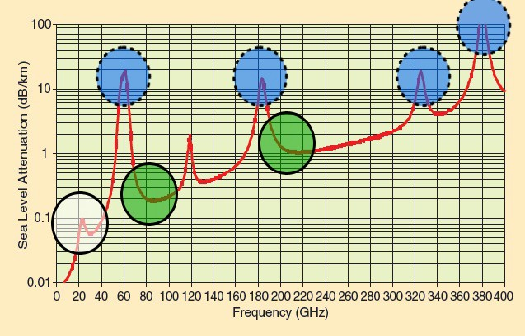
\includegraphics[width=0.7\textwidth]{Pictures/mmwave.pdf}
	\caption{毫米波频段大气衰减图\cite{rappaport2011state}}
	\label{fig:mmwave}
\end{figure}

\begin{figure}[htbp]
	\centering
	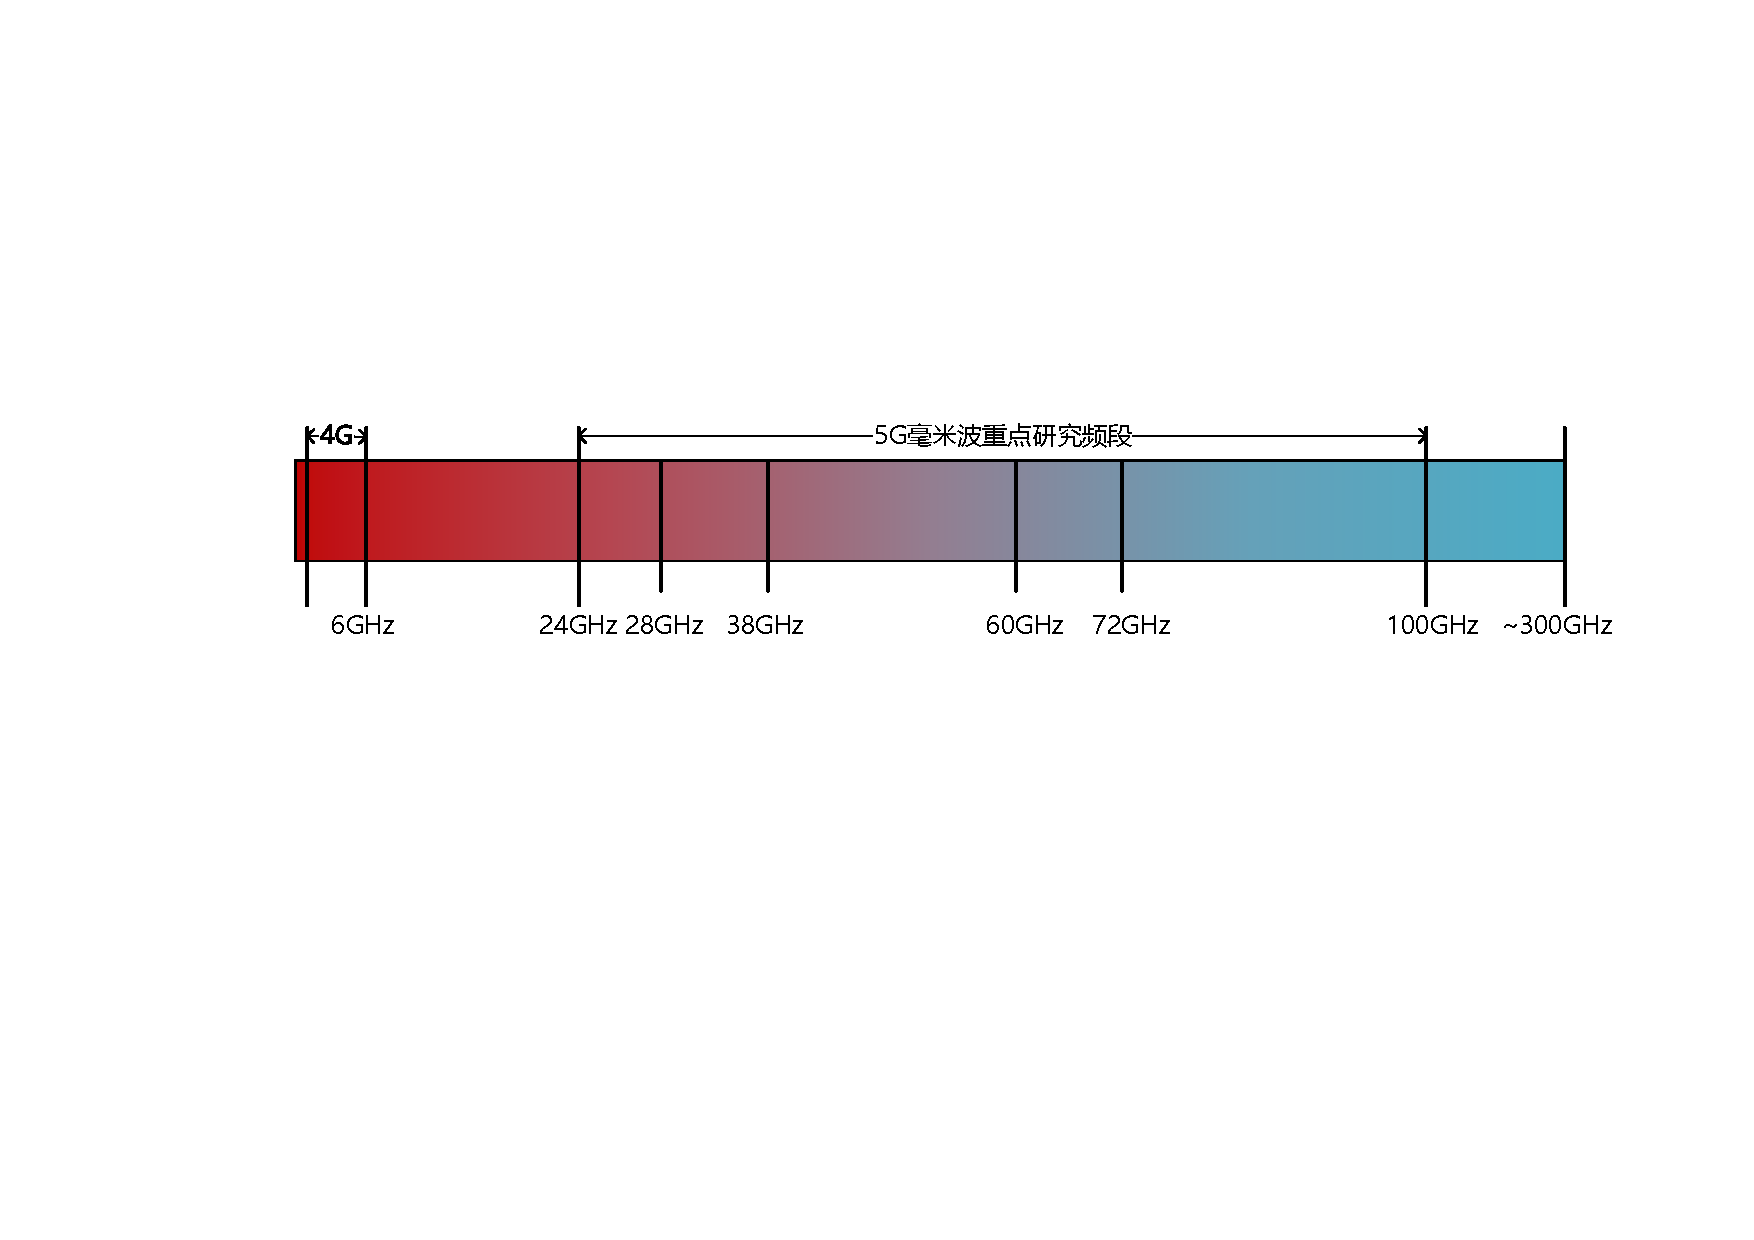
\includegraphics[width=0.7\textwidth]{Pictures/mmw.pdf}
	\caption{毫米波通信研究频谱范围}
	\label{fig:mmw}
\end{figure}

\begin{enumerate}
\item \textbf{毫米波通信技术} \quad 毫米波频段主要是指处于30-300GHz的极高频(EHF)频段,其波长在1-10毫米的范围内。该频段拥有丰富的、未被有效利用的频谱资源,能够提供高达Gbps级别的通信带宽。在传统无线通信网络中,通常是利用超高频、特高频及以下频段进行通信,而毫米波所在的极高频则通常是用于遥感卫星、射电天文学或者日常的安检扫描中,并未应用到无线数据传输领域。其原因在于虽然毫米波频段数据传输速率高,然而根据Friis自由空间衰落模型,过短的波长导致其在自由空间中的衰落速度极快,有效通信范围非常受限;同时毫米波在面对障碍物时阻挡效应严重,难以通过绕射等方式继续传播,严重影响了毫米波作为数据载体的实际应用。
近些年的研究发现,可以通过将毫米波与波束成形技术结合,将毫米波信号能量集中成方向性的窄波束进行数据传输,不但可以提高信号传输范围,还可以实现频谱资源的空分复用,提高频谱利用率;同时可以利用毫米波高速率低覆盖的特点,与致密化蜂窝小区技术结合,既可以有效地提高数据传输速率,又能避免较长的传输距离干扰其他基站小区内用户,还降低了非核心区域恶意用户的窃听机会,提高了传输数据的安全性。如图(\ref{fig:mmwave})所示为毫米波频段受大气影响的情况,在致密化小区技术的基础上,小区范围下降到200米的范围内,此时大气对毫米波的影响并不显著,尤其是在28GHz和38GHz频段\cite{rappaport2013millimeter}。现阶段毫米波通信研究主要专注在24-100GHz范围内,如28GHz\cite{pi2011introduction}、38GHz\cite{sulyman2014radio}、60GHz\cite{li2014efficient}与72GHz\cite{nie201372}等频段,见图(\ref{fig:mmw})。事实上,毫米波通信已经应用于一些无线通信标准中,如1)IEEE 802.15.3c-2009 Task Group 3c协议\cite{802153},作为第一个工作在57-64GHz频段的无线协议,首次达到了1Gbps的带宽;2)IEEE 802.11ad Wi-Fi协议\cite{80211ad},使用60GHz频段通信,最大支持32根天线,带宽可以达到4.6Gbps峰值;3)802.11ay协议\cite{80211ay,ghasempour2017ieee},作为802.11ad的继任者,是第一个真正意义上的毫米波宽带无线接入协议,它使用60GHz频段通过方向性基站进行数据传输,最高支持100Gbps的峰值传输速率,并可保证在300-500米的传输范围内得到20-40Gbps的稳定传输。

\item \textbf{波束成形技术}\quad 毫米波通信在带来更高的通信带宽同时,也带来了更快的路径衰减。为了弥补高频率带来的传输损耗,可以利用波束成形技术进行信号的发射与接收。波束成形技术建立在多天线系统的基础上,通过提高多重增益(Multiplex Gain)、分集增益(Diversity Gain)以及天线增益(Antenna Gain)以提高信号的传输效率。其中多重增益是指在多个天线上同时传输平行的多路信号,以降低误码率;分集增益是通过时空编码的方式,提高分集增益、降低误码率;天线增益是通过提高特定用户方向上的信噪比,并降低其他用户方向上的信噪比,以提高传输效率。
波束成形技术可以分为模拟波束成形技术\cite{venkateswaran2010analog}、数字波束成形技术\cite{spencer2004zero}以及混合模拟数字波束成形技术\cite{han2015large}。模拟波束成形技术通过改变每个天线单元上的信号相位,将毫米波波束能量集中到某一特定的方向上,而其他干扰方向的天线增益被显著降低,进而提高了传输的能量效率,很适合应用在室内环境的毫米波通信系统中。数字波束成形技术最早使用在传统天线数量有限的微波系统中,每个数字基带通过单独的数模(DAC)/模数(ADC)转换器控制一个天线的相位,因此相较于模拟波束成形技术能够达到更高的自由度。然而在毫米波通信中,当天线数量急速增长时,相应的硬件成本也会急剧增加,同时为每个天线单元配备一个DAC/ADC从硬件上难以实现,因此将纯数字波束成形技术用于大规模多天线阵列中并不现实。因此在未来的5G通信中,会将模拟波束成形技术与数字波束成形技术结合,利用混合波束成形技术将整个天线阵列虚拟地分成多个子阵列,每个子阵列连接在同一个射频链路上,并与一个用户进行通信。混合波束成形技术中的数字波束成形部分在基带上对信号进行预编码,当预编码过的信号通过数模转换器后,利用模拟波束成形技术将信号聚集成方向性波束与对应方向进行通信。

\item \textbf{大规模多输入多输出天线阵列技术}\quad 多输入多输出(MIMO)天线阵列系统\cite{rusek2013scaling}已经应用于现有的无线通信系统中,在4G长期演进(Long-term Evolution, LTE)标准中基站端支持最多八个天线的MIMO技术。相较于传统的单天线通信系统,在发射和接收端布置更多的天线带来了更高的自由度,更好的链接质量与更快的传输速率。MIMO技术带来了通信质量的显著改进的同时,也带来了发射接收端更高的硬件复杂度以及在信号处理中的更高的计算复杂度与能耗。5G通信系统中将MIMO系统进一步发展成为大规模(Massive)MIMO系统,在发射和接收端引入了数以百计的天线单元,以期进一步提高通信性能。在Massive MIMO系统中,天线数量将远远大于用户数量,充足的天线带来了信道硬化的特点,使得信道状态可以保持相对稳定且变化缓慢,从而使提前进行系统资源优化处理成为可能。
\end{enumerate}

\subsubsection{毫米波通信研究要点}

毫米波通信能够提供极高的通信带宽,为各种无线应用带来新的可能性,因此一直受到研究者的重视。然而毫米波信号波长过短,极易在空间中衰减,就需要利用波束成形技术将其集中成方向性波束进行传输。为了形成能量更集中、更窄的波束,需要大量的天线单元即大规模MIMO天线阵列。而大规模天线阵列的组成又是建立在毫米波信号使用的基础上:只有使用毫米波信号,天线单元的体积与单元之间的距离才能缩小到合适的范围内,进而可以将大规模天线阵列布置在发射与接收端。三者之间相互依托,密不可分。新的技术也带来了新的挑战,在这些新兴技术的支持下,如何更高效地利用系统资源提高无线通信性能,如实时性、吞吐量、能耗效率与频谱利用率等,就成为了下一代毫米波通信中重要的研究内容。本文将从三个角度进行研究,首先从毫米波方向性通信建立的基础入手,研究如何实时准确地得到多用户位置信息,以进行发射接收双方波束对准并建立连接,即毫米波通信多用户跟踪实时性问题;在此基础上,本文将研究毫米波通信在星型网络与网状网络这两类主要网络拓扑结构中的资源分配优化问题,分别将在蜂窝小区基站以及无线数据中心网络两个应用场景中进行讨论。

\begin{enumerate}
	\item 毫米波通信系统多用户跟踪实时性问题研究

	在毫米波通信系统中,极短的波长导致无线信号的衰减速度急剧增加,需要将传统的全向波转变为方向性波束以集中能量进行信号传播。毫米波只有在发射与接收波束对准的情况下才能实现其高速率的数据传输,因此毫米波通信需要需要精确的位置与跟踪信息以进行波束对准。同时由于毫米波所用天线的体积相较于厘米波段显著减小,使得将较大规模的天线布置在用户终端上成为可能。借此可以利用阵列信号处理等手段,对信号进行更准确的波达角估计,进而可以判断出与基站之间的相对方位信息,便于毫米波波束的对准与传输。同时借助空分复用等技术,基站可以在同一个频段与多个用户同时通信,这就需要同时对大量移动目标进行跟踪以便利用方向性波束通信。因此\textbf{如何提高对多个移动用户精确跟踪的实时性直接影响着用户的通信表现。}这也成为毫米波通信系统中重要的研究课题之一。在毫米波无线通信中,系统对实时性要求有了进一步的提高:感知网络(Tactile Internet)中所提出的实时性要求网络反应时间小于对应应用的某些时间常量,例如人体感知延迟的水平,即1毫秒\cite{fettweis20145g}内。因此提高对通信范围内多个目标的跟踪精度与实时性就尤为重要。本文将在毫米波通信系统中针对多个可移动用户的跟踪实时性问题进行研究。

	\item 星型网络结构毫米波通信系统资源分配与优化问题研究

	作为星型网络结构(Star Network)的典型应用之一,蜂窝移动通信系统是毫米波通信的一个主要应用场景。蜂窝系统中的基站资源管理与优化问题一直是重要的研究问题,且在引入毫米波通信等新兴技术后又出现了诸多新的挑战,如干扰对齐、绿色通信、天线分配等。系统需要对包括计算资源(运算核心)、通信资源(天线数量)、能量资源(传输功率)、频谱资源(信道分配)等在内的资源进行合理分配,以最大化系统效益。在基站-用户场景中,用户只拥有较少数量的资源而基站则拥有大量可利用资源用以分配。\textbf{如何分配基站的天线资源以提高整个系统的吞吐量}就成为了一个重要的研究问题。对此本文将在单小区单基站多用户的场景下进行研究,考虑基站端天线资源的优化问题以提高5G毫米波通信系统吞吐量等性能。

	\item 网状网络结构毫米波通信系统资源分配与优化问题研究

	此外,作为网状网络结构(Mesh Network)的典型应用之一,数据中心网络也是毫米波通信的另一个主要应用场景。该场景下通信双方都拥有较强的通信与计算能力,能够在授权或者非授权频段建立彼此之间的直接通信而无需通过基站进行数据传输\cite{asadi2014survey}。此时收发双方之间所拥有的通信资源规模相当,数据传输表现与双方都直接相关。与之前星型网络场景不同的是,在本场景中发射和接收双方可以进行同等水平的资源分配与优化。因此,\textbf{如何建立无线数据中心网络并在给定任务负荷下优化调整系统内发射接收对的通信资源以提高整个系统的通信效率}就成为一个重要的研究问题。本文将在无线数据中心网络场景下进行资源优化分配研究以提高数据中心网络的性能表现。
\end{enumerate}

\section{研究现状}

\subsection{毫米波通信系统多目标快速跟踪}

相较于传统无线通信系统,毫米波通信系统对用户定位精度和实时性要求更高。这主要体现在毫米波通信使用的是较窄的波束进行方向性通信,只有在准确的知道用户位置信息时才能进行波束对准。且用户经常处于运动中,需要在对其进行定位的同时进行波束跟踪,以提供持续性的高性能服务。由于毫米波天线阵列的特点,在只存在视距传播路径的情况下,可以进行更精确的波达角(Direction of Arrival, DoA)估计,再加以准确的到达时间(Time of Arrival, ToA)即可得到精确的用户位置信息。
Maccartney等人研究了73GHz频段毫米波信号在野外大基站小区内的传播模型\cite{maccartney2017rural,maccartney2017study},在3GPP/ITU-R的室外大基站CI模型的基础上,加入基站高度对信号传播的影响,提出了更加准确并已实施的CIH衰落模型以利于更准确的距离定位。
Savic等人提出了利用分布式Massive MIMO系统进行基于指纹的定位方法\cite{savic2015fingerprinting},在高杂波多径反射的环境中,采集用户的接收信号强度(Received Signal Strength, RSS),在只存在一个基站的情况下,利用贝叶斯非参高斯过程回归方法对用户进行高精度定位。
Koivisto等人提出了在超致密小区结构中联合设备定位与时钟同步的方法\cite{koivisto2017joint,koivisto2017high},利用基于扩展卡尔曼滤波(Extended Kalman Filter, EKF)的算法对ToA和DoA进行估计,并通过二阶段EKF对ToA和DoA进行融合估计用户位置,其提出的级联式EKF算法即使在实际工作场景下,依然能够得到移动用户米级别的定位精度以及微秒级别的时钟同步。
Cui等人提出了利用毫米波信号对车辆进行定位的方法\cite{cui2016vehicle},通过设计合适的脉冲信号波形,利用两种接收机测量时间并得到精确的位置信息,其中能量检测器消耗较低的计算复杂度,得到较高的时间测量精度;而相干接收器通过消耗更高的计算复杂度,能够得到更高的时间测量精度。

在移动通信场景中,用户通常会在一定范围内运动,因此需要在准确定位的基础上对这些移动用户进行波束跟踪,以保证基站与用户之间的连续高速率通信。通常做法在得到用户的测量位置(角度)信息后,利用各种滤波算法对收到的信息进行滤波以重新估计用户的精确位置(角度)。
日本NTT DOCOMO公司研究了在室内多反射场景下利用70GHz频段毫米波与移动性目标进行通信的问题\cite{inoue2015experimental},当用户按照$2$km/s的速度运动时,无论是在有反射或是无反射墙壁的情况,或是障碍物存在与否,系统都可以得到高达2Gbps的通信速率。
之后三星公司与DOCOMO共同研究了在户外场景下利用28GHz频段毫米波超宽带无线信号与高移动性用户进行通信的问题\cite{obara2016experiment},在基站使用48个天线单元组成的平面天线阵列,通过混合数字模拟波束成形技术将毫米波信号将极窄的波束发射到拥有4个天线组成的均匀线性阵列的移动设备上。实验证明了即使用户在处于$60$km/s的运动速率时也能够得到约4Gbps的高通信速率。
Tateishi等人研究了在室内场景下利用15GHz频段对移动目标进行波束跟踪的问题\cite{tateishi2016indoor},证明了即使存在丰富的多径路径情况下,用户仍然能够在50米的距离达到7.7Gbps的峰值下行速率。
Kim等人研究了在OFDM毫米波无线通信系统中的波束跟踪问题\cite{kim2018beam},在多小区多用户的场景中,设计将基站天线阵列分成两个子阵列,通过特殊的导频设计可以区分不同的子阵列的信号,并计算两者的相位差得到波束发射角(Angle of Departure, AoD)与波束到达角(Angle of Arrival, AoA)并以此进行多用户跟踪。
Suhanya等人提出了一种鲁棒性的波束跟踪算法\cite{jayaprakasam2017robust}。在固定的基站运行扩展卡尔曼滤波,并通过EKF估计出的误差协方差来鲁棒地更新波束成形权重。
Vutha等人研究了在模拟波束成形场景中通过只训练一个波束对来跟踪一条轨迹的方法\cite{va2016beam},此设计同样也利用了扩展卡尔曼滤波作为跟踪滤波算法,并证明了在同样的信噪比情况下,较窄的波束对角度改变更加灵敏,因此能够提供更高的跟踪精度,然而过窄的波束也同时容易导致波束错位,降低跟踪的精度。
Yu等人则研究了在慢衰落MIMO干扰信道中波束跟踪对于干扰校准的影响\cite{yu2012beam},通过应用矩阵扰动理论混合特征分解和预测过程以最小化干扰校准预测步骤的复杂度,该算法能够使用更低的计算复杂度得到与传统算法相似的跟踪效果。
Wei等人提出了利用毫米波无线射频进行高精度无源用户跟踪的方法\cite{wei2015mtrack},并将跟踪精度提高到了分米的级别,通过高方向性的60GHz毫米波波束扫描发现用户的初始位置,并降低环境中背景反射造成的干扰,最后利用基于信号相位的模型对用户路径进行跟踪。

在毫米波通信系统中,大部分研究工作关注单目标的定位与跟踪问题,很少涉及到多目标跟踪领域;且多着重于跟踪精度提升,对跟踪实时性研究较少。本文着眼于毫米波通信中的多目标跟踪实时性问题,为毫米波通信建立位置信息基础。

\subsection{毫米波蜂窝系统基站资源分配与优化}

蜂窝小区网络是毫米波通信的重要应用场景之一,其主要由基站及众多用户组成,是一种典型的星型网络拓扑结构。现有蜂窝网络技术中引入了MIMO技术,利用多个天线组成的天线阵列,通过空时编码与波束成形等技术实现了空间分集和空间复用,提高了信道频谱利用率。
在引入毫米波通信后,为了进一步提高天线系统的增益,美国贝尔实验室的科学家 Marzetta 在MIMO技术的基础上,于2010年最早提出了适用于毫米波通信的Massive MIMO天线系统概念\cite{marzetta2010noncooperative}。假设在一个时分双工无线通信系统中,基站拥有无限数量的天线资源,即可在同一个时间频率上与多个用户分别通信。之后Rusek等人认为在目前的理论研究及硬件实现中,可以定义大规模MIMO系统中的基站天线数量在100到1000个天线终端范围内\cite{rusek2013scaling},同时该系统符合随机矩阵理论中的一些渐进结果,例如信道中的奇异值分布会趋向于具有确定性的函数等。不仅如此,使用大规模MIMO阵列天线还可以大幅度提高频谱与能量利用效率\cite{lu2014overview}。由于系统采用TDD的方式,上下行信号在同一个频段内通信,在很短的时间内可以认为上下行信道是具有相互性(Reciprocal)\cite{bjornson2016massive}的,即两个方向上的信道响应是相同的。可以通过上行信号的信道响应得到信道状态信息(Channel State Information, CSI),并对上下行信道进行估计,因此可以通过增加基站天线数量来提高系统性能\cite{marzetta2006much}。在多基站多小区的情况下,由于正交信道导频数量远小于用户数量\cite{marzetta1999blast},相邻基站用户非正交导频会带来导频污染问题。但是当基站天线数量无限增长时,会出现信道硬化(Channel Hardening)\cite{hochwald2002space,hochwald2004multiple}的特性,非相关噪声与快速衰落效应都将消失,只剩下由于导频污染导致的小区间干扰影响系统表现,随机的无线信道特性趋向于确定\cite{wangxinshui}。在此基础上,Hoydis等人\cite{hoydis2013massive}研究了当Massive MIMO系统中基站天线数量相较于用户数量并非无穷大时的系统表现,并给出了计算每个用户需要多少数量的天线以满足一定比例的无限天线系统极限表现的方法。同时证明了通过最小均方误差法(MMSE)和正则迫零法(RZF)可以在节省较多天线资源的同时达到特征值波束成形法与匹配滤波所能得到的效果。在这类场景中可分配资源通常包括天线资源、用户配对、信道分配或是能量分配等。而其优化目标一般为最大化系统吞吐量、频谱利用效率、能量利用效率或是最小化通信误差等目标。

在频谱资源优化方面,4G中主要使用正交频分复用(Orthogonal Frequency Division Multiple Access, OFDMA)技术\cite{holma2009lte}。在5G的研究中,除计划继续使用TDMA、FDMA或OFDMA等正交方法之外,有研究认为可以采用如半正交多址接入SOMA\cite{khormuji2015generalized}、稀疏编码多址接入SCMA\cite{nikopour2013sparse}、交织多址接入IMDA\cite{ping2006interleave}等非正交多址接入(Non-orthogonal multiple access, NOMA)类技术\cite{saito2013non,dai2015non},将多个用户的信号在能量域上叠加,在接收端利用连续干扰消除的方法逐步提取目标信号,此时所有用户可以在相同的时间使用相同的频率与编码进行通信,这将极大提高系统频谱利用率。

在能量利用效率方面,毫米波通信系统中的绿色通信被列为重点研发方向。事实上电力资源消耗是通信运营公司的主要运行成本,因此提高毫米波无线传输能量利用效率具有重要的研究意义。
Bj{\"o}rnson等人研究了如何在Massive MIMO系统中得到最优的能量利用效率\cite{bjornson2015optimal},提出了最优能量效率与天线数量、活动用户数量以及发射功率之间的闭式关系。
Ngo等人证明通过使用Massive MIMO系统可以提高频谱利用率的同时更好的提高能量利用率\cite{ngo2013energy},只需通过MRC,ZF等简单的线性过程,通过对上行导引向量进行信道估计即可降低小区内的干扰,同时权衡了频谱利用率与能量利用率以得到最优的系统收益。
Shi等人则研究了多小区Massive MIMO系统的小区上行覆盖范围优化问题\cite{jin2015cell}。通过应用在基站上的倾斜可调整的天线阵列可以优化小区覆盖范围,中和小区边缘覆盖与导引向量污染的问题。同时文章对不同小区形状以及用户性质的情况进行了分析,通过简单的线性查找即可得到最优覆盖方式。
为了得到准确的信道状态信息,大部分工作都将研究注重于时分双工系统,即上下行信道只有时域上的区分,在频域上保持有相互性。然而Adhikary等人研究了在移动通信中普遍使用的频分双工(Frequency Division Duplexing,FDD)系统\cite{adhikary2013joint}中的CSI问题。由于不能利用上下行信道的相互性,系统需要利用联合空间分集与复用技术(JSDM)在FDD通信系统中获取即时信道状态信息,并借此方法只需通过较少的二阶统计信息即可得到有效地空间分集增益。

现有研究工作中大部分都针对传输信道、能量以及波束成形权重等要素进行资源优化,很少有针对大规模天线阵列本身天线单元的资源优化研究。随着阵列天线上天线数量的增多,天线单元本身也成为需要优化分配的重要资源。本文将针对蜂窝小区基站天线阵列中天线资源本身及其子阵列形状适配等优化问题进行研究。

\subsection{毫米波无线数据中心网络资源分配与优化}

数据中心网络(Data Center Network,DCN)是毫米波通信的另一个重要应用场景,也是一种典型的网状网络拓扑结构。随着大数据、云计算、人工智能、超级计算等新技术在各个领域的运用越来越广泛,数据中心对海量数据的储存与传输变得越来越重要。其中数据中心网络通过电缆、光纤和无线等方式建立高效的拓扑结构,将多种物理单元连接起来,负责着极为重要的通信功能。

早期的数据中心网络流量主要以南北向流量(North-South Bandwidth)为主,即数据中心外到数据中心服务器之间进出的流量。然而随着大数据等科技的应用,东西向流量(East-West Bandwidth)即数据中心服务器之间的流量越来越重要。 按照Cisco公司发布的全球云指数白皮书\cite{cisco2018cloud}预测,到2021年$85\%$的数据中心流量将会是服务器之间或数据中心之间的东西向流量,而服务器与外界互访的南北向流量将会下降到$15\%$左右。许多很小的应用将会需要动态调动大量的数据传输,传统的多层数据中心网络将难以满足强大的传输带宽需求。因此有研究者考虑使用灵活性更高的无线方式动态地进行服务器/机架间的点对点通信,以降低通信热点的发生,降低系统传输时延。

有线数据中心网络主要分为两大类,一类是简单的树状结构,在接入层使用接口较少的廉价交换机,汇聚层使用接口较多也更昂贵的交换机,而在核心层使用拥有数百个万兆接口的极为昂贵的高性能交换机以满足数据分发的需要。这种结构对核心层网络设备有极高的性能要求,而且当服务器数量和拓扑结构发生改变时,难以满足可扩展性的需求,同时容易带来带宽超额(oversubscription)的问题。

\begin{figure}[t]
	\centering
	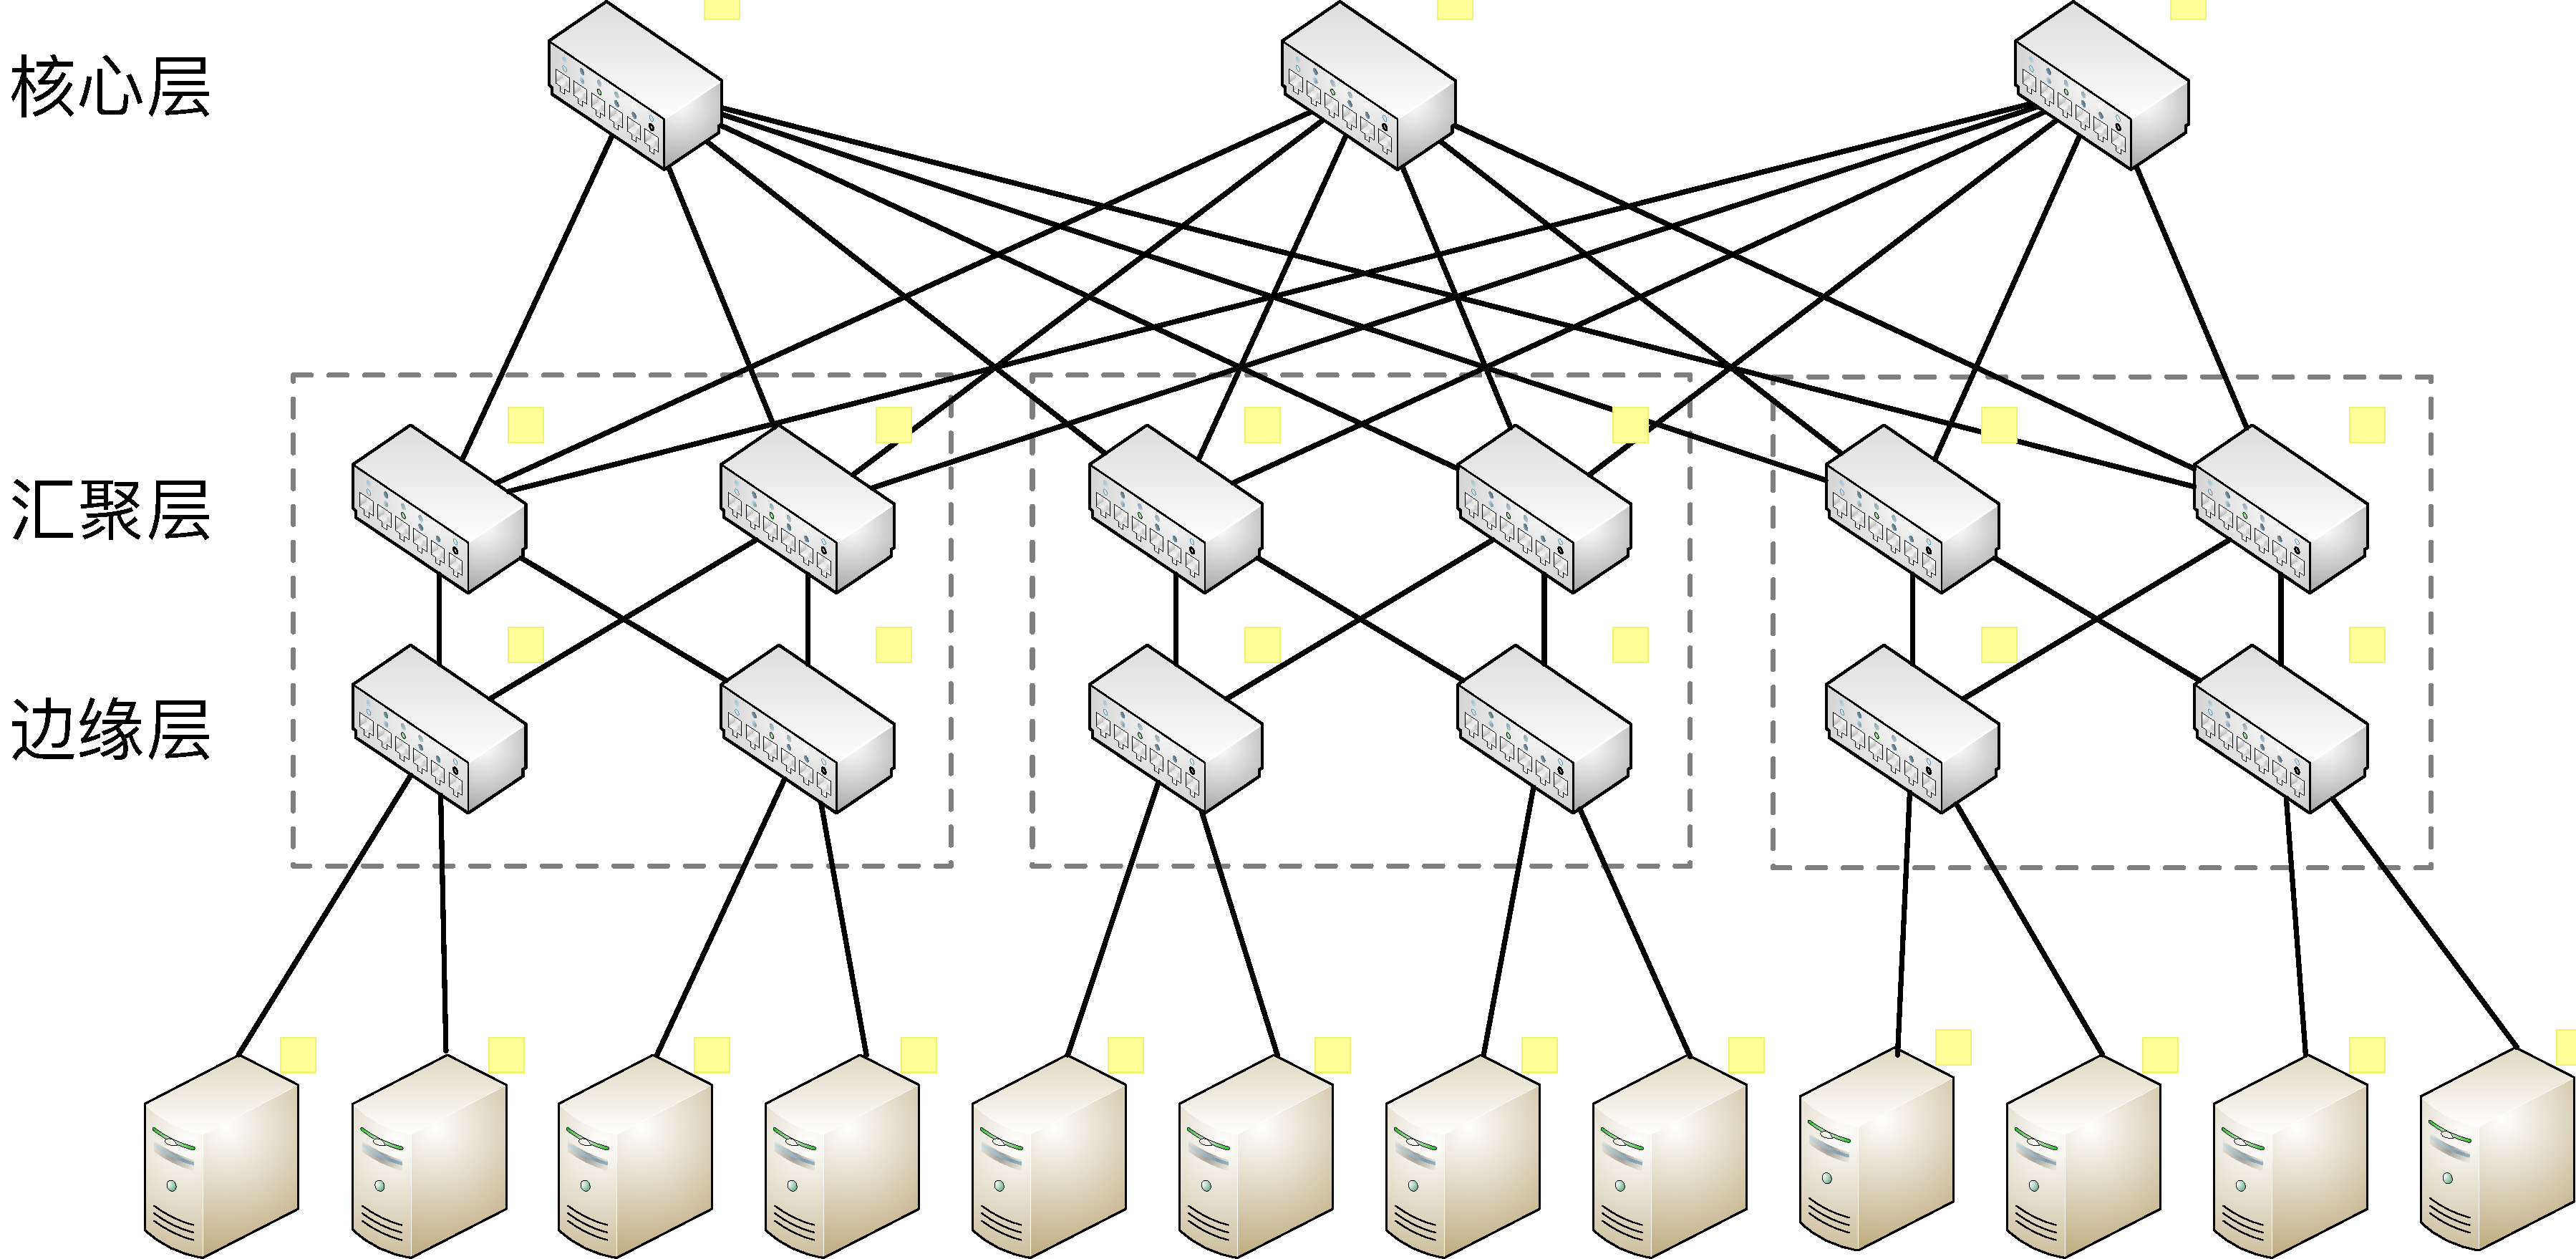
\includegraphics[width=0.7\textwidth]{Pictures/fattree.pdf}
	\caption{Fat-tree数据中心架构示意图}
	\label{fig:ft}
\end{figure}

\begin{figure}[t]
	\centering
	\includegraphics[width=0.7\textwidth]{Pictures/helios.pdf}
	\caption{Helios数据中心架构示意图}
	\label{fig:helios}
\end{figure}


现有的数据中心网络主要为分级的互联网络结构,利用交换机将各个物理结构进行连接\cite{xia2017survey,chen2016features}。通常是一种分级的胖树(Fat-tree)型互联模型网络架构,通过加入冗余的带宽和交换机阵列,使用经济的平价交换机代替昂贵的高性能交换机,同时冗余交换机的引入也缓解了单点失效的问题。

传统的有线数据中心网络一般主要包含三层:核心层(Core Layer)、汇聚层(Aggregation Layer)和接入层(Access Layer)。
\begin{enumerate}
	\item 核心层负责数据中心流入流出的路由功能,提供与大量汇聚节点的丰富连接。
	\item 汇聚层提供核心层与接入层之间的连接,同时也提供防火墙、负载平衡、流量汇聚与应用加速等服务。
	\item 接入层连接服务器与数据中心网络,是整个架构中最底层的结构。
\end{enumerate}

多余的冗余交换机在带来对等带宽的同时也带来了巨大的资源消耗,如图(\ref{fig:ft})所示。主要包括三种类型,以交换机为核心的架构(Switch-centric topologies),以服务器为核心的架构(Server-centric topologies),以及各种增强型架构。
在以交换机为核心的架构中 \cite{singla2012jellyfish,walraed2013aspen},交换机处于多层级架构中的高层位置,而服务器处于网络边缘较低层的位置。
Fat-tree拓扑结构 \cite{al2008scalable}是在传统树形结构的基础上改进的三层拓扑结构。在Fat-tree架构中,系统主要由自上而下的核心层、汇聚层和边缘层构成,边缘层与服务器相连。各层级的交换机为同型号交换机,且每个节点的上下行带宽保持相等。同时对于任意两个服务器之间都有着多条相同代价的传输路径,因此理论上可以得到完全对等的带宽。然而这种架构使得交换机之间的接线非常复杂且冗余。
VL2 \cite{greenberg2009vl2}是与Fat-tree类似的三层树状拓扑结构。只是每个边缘层交换机都与两个汇聚层交换机相连,而汇聚层与核心层之间的交换机则以完全二部图的形式相连接。在提高了交换机之间线缆带宽的同时减少了总体线缆数量。

在以服务器为核心的模块化数据中心架构中,服务器吸纳了更多的连接与路由功能,除了作为拓扑网络中的终端节点外,更成为彼此间的中继节点。作为组网与路由的核心,服务器的作用变得更加重要,交换机则只作为单纯的数据转发。微软亚洲研院在2008到2013年间陆续提出了DCell\cite{guo2008dcell}、FiConn\cite{li2009ficonn}、BCube\cite{guo2009bcube}、MDCube\cite{wu2009mdcube}以及CamCubeOS\cite{costa2013camcubeos}等数据中心网络拓扑架构。
其中DCell\cite{guo2008dcell}是一个典型的以服务器为核心的递归型数据中心拓扑架构。在最底层的0-层,有n个服务器直接与一个交换机相连;这样的n+1个0-层结构构成了1-层DCell架构,每个0-层结构中的服务器提供一个端口与另一个0-层结构中的服务器相连,若将0-层结构看做是一个虚拟节点,则整个1-层形成一个完全图网络。因此DCell结构提供了很强的可扩展性。然而此架构中网卡数量指数级增长,且系统仍为有阻塞的架构。
FiConn\cite{li2009ficonn}则考虑到实际系统中,服务器与交换机的物理网卡接口数量的限制,将服务器端的物理网卡接口数量设置为2个,在此基础上以多层递归的形式将网络连接起来,这可以被认为是低连接度版本的DCell架构。与DCell类似,FiConn也是由相同的基本单元构成的递归型架构,相较于DCell减少了大量的网络传输线路,也降低了布线的难度。
BCube\cite{guo2009bcube}可以看作是集装箱式的模块化数据中心结构。它与DCell架构类似,也是一个递归型的以服务器为中心的拓扑架构。在0-层架构中与DCell相同,也是有n个服务器直接与一个n接口交换机相连;在上层的k-层结构中,都由n个k-层结构组成,每个交换机与每个(k-1)-层中的服务器相连。可以认为BCube是Fat-tree与DCell权衡后的结果:相较于Fat-tree结构而言,BCube节省了交换机的数量,但是增加了网卡数量,并能够提供更好的一对多服务;而相较于DCell而言,BCube提高了网络转发效率,能够提供更高的网络容量。
MDCube\cite{wu2009mdcube}则是将多个BCube连接起来,已适用于超大规模数据中心网络。其引入带宽更宽的光交换机用于BCube集装箱式模块之间的通信,而BCube集装箱式模块之内的通信仍使用传统电交换机。

随着数据量的极速增长以及服务器间数据流量的增加,数据中心对传输带宽的要求逐渐升高,传统的电缆连接已渐渐不能满足高速数据中心网络的需求;同时随着商业光通信交换机设备的价格逐渐降低,基于光信号传输的系统架构映入研究者的视线。光交换机可以有选择地将光纤中的光信号进行转发,能够提供巨大的传输带宽。现有工作主要是将光信号交换机与现有电信号交换机混合组网,以提高传输速率。一般而言,电信号交换机通常仍组成树状结构,而光交换机则采用单跳的方式连接两个服务器。

早在2005年Barker等人就提出利用光路交换机\cite{barker2005feasibility}降低数据中心网络的通信成本。在高性能计算机系统中建立两套通信网络,一套利用光路交换机(OSC)价格便宜且能耗较少地满足长期且大量的数据交换,另一套则使用电包交换机(EPS)用来满足短期的低带宽数据交换。光路交换机系统使用了较少的光学传输设备,能够显著的降低数据中心网络成本。
Wang等人引入了基于MEMS的光学交换机\cite{wang2009your},组成混合包交换/电路交换网络。设计可以提供更易用的全数据包网络,同时低成本地为一些高级的应用提供了更高的带宽。
Helios\cite{farrington2010helios}提出了混合电子/光学交换机架构,可以大量减少交换机数量、线缆和能源消耗等,这是一个2层的多根树状结构,利用被动光学分路器(Mux)承载不同波长的信号进行高容量的单跳通信,并通过最大最小公平进行带宽的估计,如图(\ref{fig:helios})所示。
2011年Wang等人提出c-Through\cite{wang2011c}在原有有线数据中心网络的架构中,引入了高带宽低复杂度的MEMS机架间光路交换机。通过波分复用技术(Wave Division Multiplexing, WDM)显著提高了总通信带宽。提高了数据中心网络的通信带宽。
Helios与c-Through的区别在于Helios在交换机上进行流量估计与流量多路分解,而c-Through则在服务器端进行流量控制。 c-Through的优势在于可以通过服务器进行数据缓冲,并打包将数据进行转发,使得光学路径传输更加高效。
Helios在交换机上实现流量估计与多路分解的工作,虽然使得整个流量控制对终端透明,但是需要更新所有的交换机设备。而c-Through则将数据缓冲在终端设备上。两者体现了在混合有线数据中心网络设计上不同的权衡方式。
OSA\cite{chen2014osa}在c-Through和Helios的基础上建立光路单跳网络,依靠Hedera\cite{al2010hedera}在理想无阻碍网络中进行基于最大最小平等带宽分配方式分配TCP流量。进而通过多个单跳连接缝合技术建立所有服务器间的通信网络。此外还可以动态调整光路链接的带宽,以更细粒度地适应数据传输需求。
Sun等人提出了基于Fat-tree模型的改进的Diamond\cite{sun2014diamond}结构。它用边缘交换机替换掉Fat-tree模型中所有汇聚层的交换机,并将边缘交换机与核心交换机直接连接。相较于Fat-tree模型,通过此方法可以有效的降低端到端(End-to-End)的时延。
最新的一些研究已经开始使用毫米波无线通信加强数据中心网络,其中包括使用喇叭状天线\cite{halperin2011augmenting},或是阵列天线3D波束成形\cite{zhang20113d,zhou2012mirror}等技术建立点对点无线链接。

现有研究工作主要通过建立新型拓扑结构等方式对数据中心网络进行优化。在引入毫米波通信后服务器间的通信变得更加多样化与自由化,预期可以极大的提升网络性能。利用毫米波高速通信建立无线数据中心网络架构的研究方兴未艾,本文中也提出一种基于阵列天线的点对点视距通信毫米波无线数据中心网络设计,并对其阵列天线资源进行优化分配研究。与星型网络不同,这种网状网络中任意两者之间都有可能发生通信,通信的双方所拥有的资源处于着相同的水平且不需要通过基站建立通信。此时只针对基站等资源优势的一方进行资源分配与优化难以得到系统的最优解,需要同时对发射与接收双方进行资源的分配与优化。

\section{本文研究内容}

\subsection{研究思路}

本文研究在下一代毫米波无线通信系统中的资源分配与优化问题。全文的思路和基本组织结构如图(\ref{fig:the})所示。第一章介绍了下一代毫米波无线通信系统,及其相关的多目标跟踪实时性与资源优化分配问题的研究背景及研究现状;第二至四章为本文的主体部分,其中第二章研究了毫米波无线通信系统中多目标跟踪实时性问题,提高了用户位置信息获取的实时性,为后续第三、四章不同网络拓扑场景下的毫米波通信建立了基础;之后第三章研究了星型网络拓扑下的毫米波通信资源分配问题,主要针对蜂窝小区中基站侧天线资源进行优化;接着在第四章研究了网状网络拓扑下的毫米波通信资源优化分配问题,主要针对无线数据中心网络中机架天线资源进行优化;第五章对全文做了总结与展望。

\begin{figure}[t]
\centering
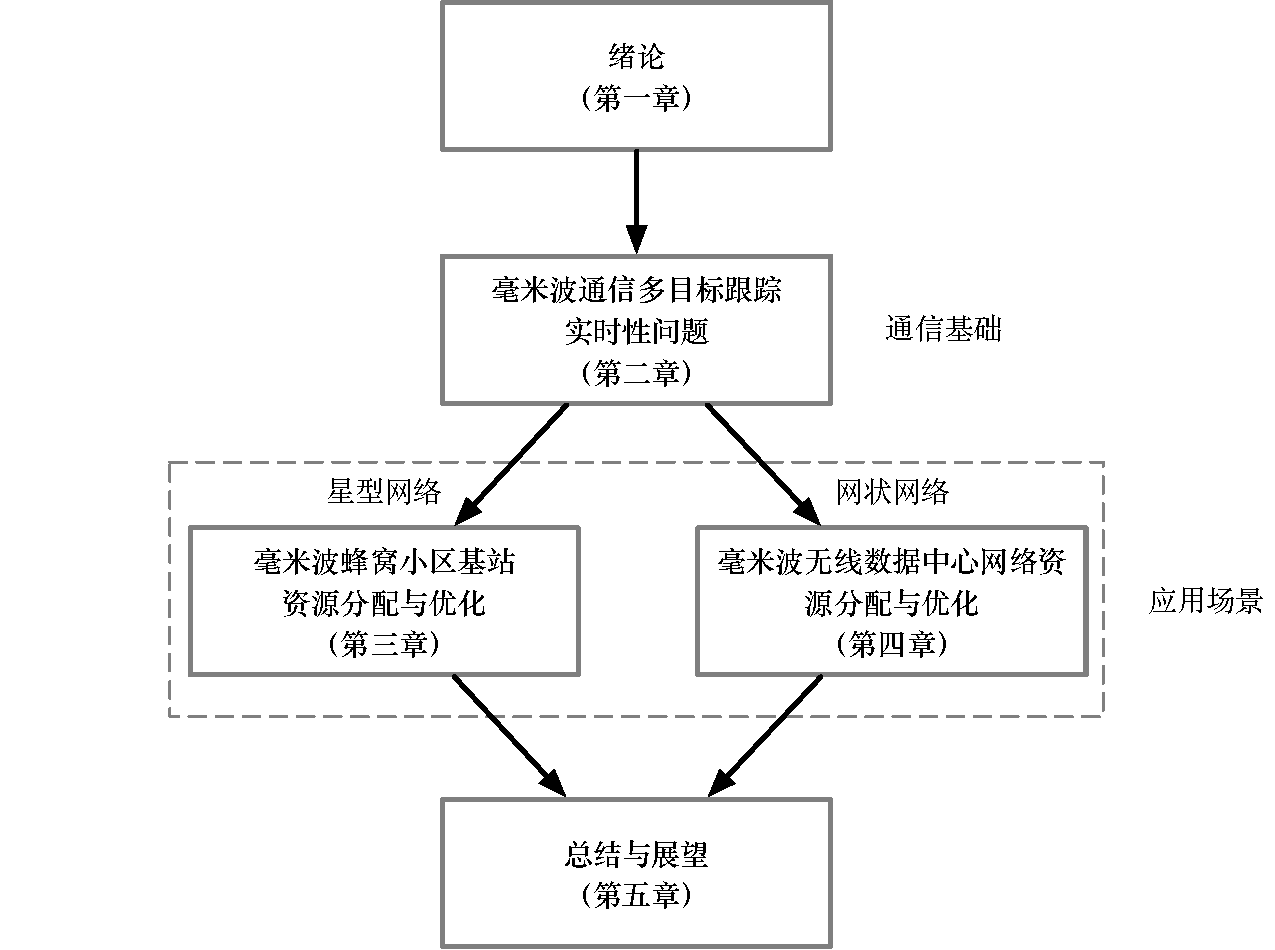
\includegraphics[width=0.9\textwidth]{Pictures/zongjiegou.pdf}
\caption{全文组织结构}
\label{fig:the}
\end{figure}

\subsection{研究内容}

本文的具体研究内容如下:

第二章研究了毫米波通信系统中的多用户快速跟踪问题。由于毫米波通信与波束成形技术的引入,基站会通过很窄的波束与用户进行通信。精确的用户位置信息能够帮助更好地进行波束对准,因此基站需要准确地感知并估计小区内处于移动中的用户的个数及其各自位置信息,这就是一个多目标跟踪问题。同时,准确而快速的跟踪意味着更低的通信时延,因此毫米波通信中多目标跟踪的实时性也亟需提高。现有的高效多目标跟踪算法,如概率假设密度粒子滤波算法等,由于其中重采样算法的限制,难以做到流水线化计算,制约了实时性的进一步提高。本章提出一种改进的重采样算法,通过引入粒子复制序列集合以及待复制粒子序列,使得需要重采样的粒子在只获得自身信息与之前重采样粒子信息的时即可进行粒子复制运算,而不用等待所有粒子完成权重值过滤后才能继续重采样。通过引入此改进的重采样算法,整个概率假设密度粒子滤波算法能够实现完全流水线化的运算。在此基础上,本文提出基于多核处理器硬件平台的计算资源分配优化算法,通过解决一组混合整数规划问题,得到了高时效的近似解法。仿真结果验证了提出的算法在保证跟踪精度的情况下,能显著降低整个滤波算法的计算时延,有效地提高了用户跟踪的实时性,为基站中每个用户的低时延通信提供了保证。

第三章研究了毫米波通信在星型网络拓扑下的典型应用——蜂窝小区网络中的资源优化问题。基站在已知小区内多个用户位置的情况下,优化分配资源以最大化系统收益即吞吐量。基站上的大规模天线阵列虚拟的分成若干个均匀线性子阵列,分别通过波束成形技术与对应的用户进行通信。由于大规模天线阵列与每个均匀线性子阵列都有着一定的固定的形状,因此问题建模为如何在矩形阵列中合理的放置这些子阵列,使得系统收益最大,这既需要考虑每个用户所占用子阵列的天线的数量,又需要考虑这些子阵列在矩形阵列中的位置分配。此场景根据不同的子阵列放置方式,又包含了两种不同的情况:1)所有线性子阵列都互相平行且平行于矩形阵列的一条边;2)为了进一步提高系统收益,线性子阵列可以平行于矩形阵列的任意一条边,即存在相互垂直的子阵列。对两种情况分别进行问题建模,对两个NP难问题进行分解并逐步求解。通过解决一系列的多选择背包问题,多背包问题和带状装箱问题,得到了两种情况下多项式时间的近似算法,并给出了每个算法的计算复杂度和下界。仿真结果验证了提出的两种算法在不同的情况下都能有效地分配天线资源,得到有性能保证的系统收益。

第四章研究在毫米波通信在网状网络拓扑下的典型应用——无线数据中心网络中的资源优化问题。在下一代数据中心网络中利用毫米波高速无线传输代替传统服务器间有线连接,以提高数据中心网络灵活性及可扩展性等。随着数据流量特性的变化,网络中出现了流量极度不平衡现象,降低了整个网络的通信性能。数据中心的机房环境相对稳定,服务器间位置也相对密集且固定,因此可以通过60GHz毫米波无线通信建立服务器间点对点直接连接,减小通信热点带来的通信性能下降。设计在每个服务器机架顶(Top of Rack, ToR)布置毫米波天线,并提出适用于阵列天线的点对点视距通信六边形机架布置方案,同时建立了单层和三层的数据中心无线网络拓扑结构,提出了对应的网络节点与边生成方式。进而对建立的无线数据中心网络结构提出了天线资源优化分配问题,通过变量替换等方式将其转化为一几何规划问题进行求解。仿真结果验证了所提出毫米波无线数据中心网络结构与优化算法能够有效降低系统的最大通信时延。